\chapter{Holmberg Equation}\label{holm}
Erik Holmberg (1946) established a simple galaxy model which we have used in the study of spin vector alignment. The two major axes in the main plane are of equal size a, the polar axis is the smallest one denoting the relative thickness of the ellipsoid. It has lenght $q\,a$, $q$ being the so called flatness factor, a number $\in$ [0,1] corresponding to the relative thickness of real spiral galaxies. Holmberg (1946) suggested a value of $q$= 0.2.
\section{Relation Between The Inclination And The Axial Ratio}
Holmberg equation is the relation between the axial ratio, $\frac{b}{a}$ and the inclination angle $i$, angle measured between the line-of-sight and direction perpendicular to the plane defined by the two major semi axes.
\begin{figure}
\centering
	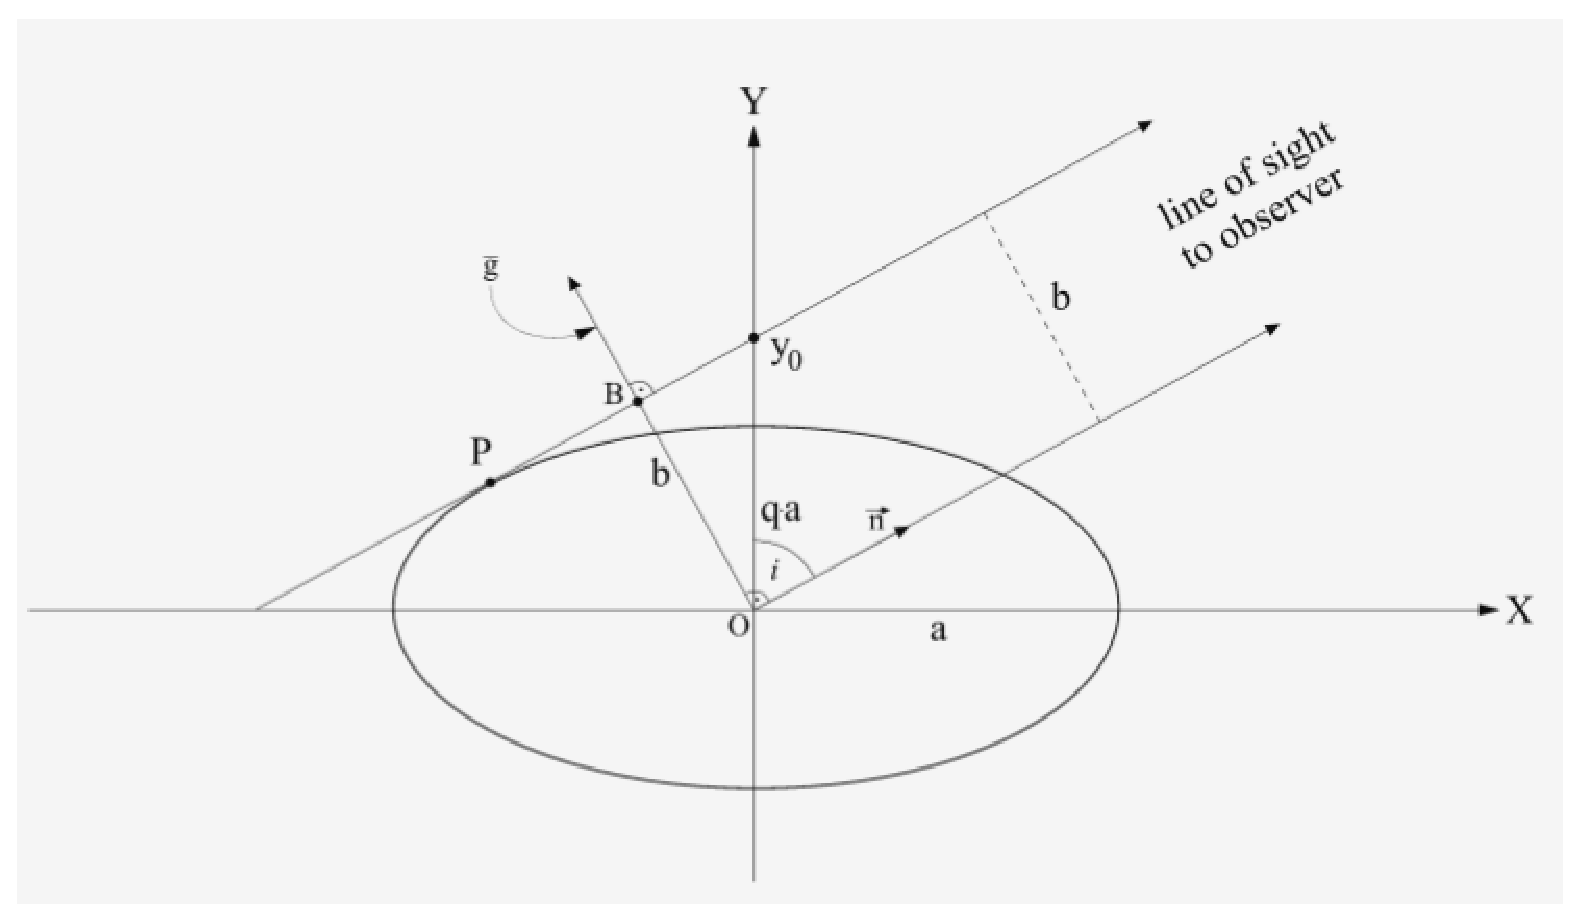
\includegraphics[height=6cm]{hom.eps}
	\caption{Derivation of Holmberg equation. (Hubble E. 1926)}\label{hom}
\end{figure}
Fig \ref{hom} shows the oblate spheroid aside, so an ellipse with an eccentricity of 0.2 is drawn. The celestial plane is perpendicular to the paper plane, intersection line is denoted by $\bar{g}$.\\\\
Fig \ref{hom} also shows the line of sight to the observer, the inclination $i$ is measured between this line and the Y-axis. This angle can be found between $\bar{g}$ and the -X-direction.\\\\
The equation of the ellipse is
\begin{equation}\label{ellipse}
q^2\,x^2 + y^2 = a^2\,q^2
\end{equation}
From the observers point of view the oblate spheroid seems to be projected onto the celestial plane as an ellipse. The quantity b, the connecting line $\bar{OB}$, is the small semi axis of this ellipse, the large semi axis $a$ of which is independent of the projection, so it is same as the one of oblate spheroid.\\\\
Assume a tangent in point $P$. The equation of the tangent is \begin{equation}\label{tangent}y=k\,x + y_0\end{equation}The condition for contact to the ellipse in Fig \ref{hom} is determined by applying the condition that \eqref{ellipse} and \eqref{tangent} touches each other. i.e 
\begin{equation}
a^2\,k^2 + a^2\,q^2 = y_0^2
\end{equation}
beging $k\,=\,cot\,i$ the slope of the tangent and $y_0$ the intersection of the tangent wiht the Y-axis.\\\\
This can be used to determine $y_0:$
\begin{equation}\label{red_cond}
y_0^2 = a^2 \cot^2\,i + a^2\,q^2
\end{equation} 
Using $b=y_0\,\sin\,i$ in \eqref{red_cond} we get
\begin{equation}
\sin^2 i=\frac{\frac{b^2}{a^2}-1}{q^2-1}
\end{equation}
which leads to
\begin{equation}\label{holmberg_equation}
\cos^2 i=\frac{\frac{b^2}{a^2}-q^2}{1-q^2}
\end{equation}
\eqref{holmberg_equation} is called \textquoteleft Holmberg Formula\textquoteright. It can be seen that there is a strong nonlinearity at large diameter ratios. The small measurement errors in teh semiaxes produce large deviations in the resulting inclinaiton angle.
\begin{figure}[H]
\begin{center}
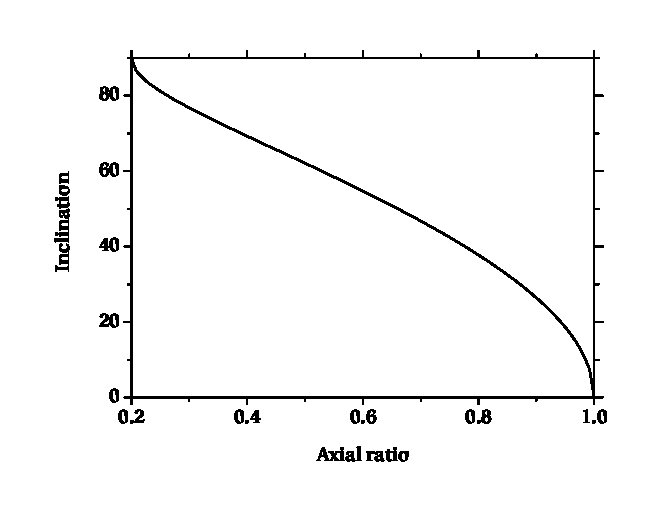
\includegraphics[height=6cm]{holmberg.eps}
\end{center}
\caption{Plot of the Holmberg Function: There is a strong nonlinearity at the lower
and the upper end of the diameter ratio interval. The flatness factor q = 0.2}
\end{figure}